% 3. Protokoll

% Variables
\def\skalierung{0.65}

\chapter{Messprotokoll}
\label{chap:protokoll}

\section{Vorarbeiten}
\label{sec:vorarbeit}

Der Versuchsaufbau wurde schon für die Versuchsteilnehmer komplett aufgebaut. Nur der Chopper musste so eingestellt werden, dass der Strahlengang nicht durch die Jod-Probe läuft. Der Versuch wird hier auch nur mit der Jod-Probe durch geführt. Die meisten Messwerte werden vom Oszilloskop ausgemessen, wobei dabei wurde immer ein Fehler von $\pm$ 5\,mV bei kleinen Bildern und $\pm$ 3\,mV bei großen Bildern angenommen. Zudem ist anzumerken, dass die Modulationsfrequenz $\omega_\mathrm{m}$ als fehlerfrei angenommen wird und deshalb keinen Messfehler besitzt.

\section{Freier Spektralbereich}
\label{sec:specBereich}

Zuerst wird der freie Spektralbereich mit dem Oszilloskop gemessen. Dafür wird die $\omega_\mathrm{m}$ auf dem Oszilloskop so eingestellt, dass von zwei benachbarten Resonanzordnungen die positive und die negative Seitenlinie übereinanderliegen. Dafür wird am HF-Generator (Hochfrequenzgenerator) eine Frequenz so eingestellt, dass sich die positive und negative der zwei benachbarten Seitenbanden überlappen. Damit ergibt sich der freie Spektralbereich aus dem doppelten eingestellten Modulationsfrequenz $\omega_\mathrm{m}$. 
\begin{gather}
    \omega_\mathrm{m} = ( 1008,5 \pm 5 )\,\mathrm{MHz} \\
    \mathrm{FSR}_\mathrm{HF} = 2 \cdot \omega_\mathrm{m} \\
    \Rightarrow \boxed{\mathrm{FSR}_\mathrm{HF} = ( 2017,0 \pm 5 )\,\mathrm{MHz}}
\end{gather}

Auf den Oszilloskop (OS) wird dann für den freien Spektralbereich eine Frequenz von 
\begin{gather}
    \boxed{\mathrm{FSR}_\mathrm{OS} = (51 \pm 2)\,\mathrm{Hz}~ = (19,7 \pm 0,5)\,\mathrm{ms}.}
\end{gather}

\subsection*{Fehler bei Bestimmung des freien Spektralbereichs}

Bei der Bestimmung treten Fehler der optischen Art auf, da hier nur mit dem Auge auf dem Display des Oszilloskop abgeschätzt wird, wie die Seitenbanden überlappen. Durch verändern der Modulationsfrequenz wurde ein ungefährer Fehler abgeschätzt.

\begin{center}
    \captionsetup{type=figure}
    \begin{tabular}{c c}
        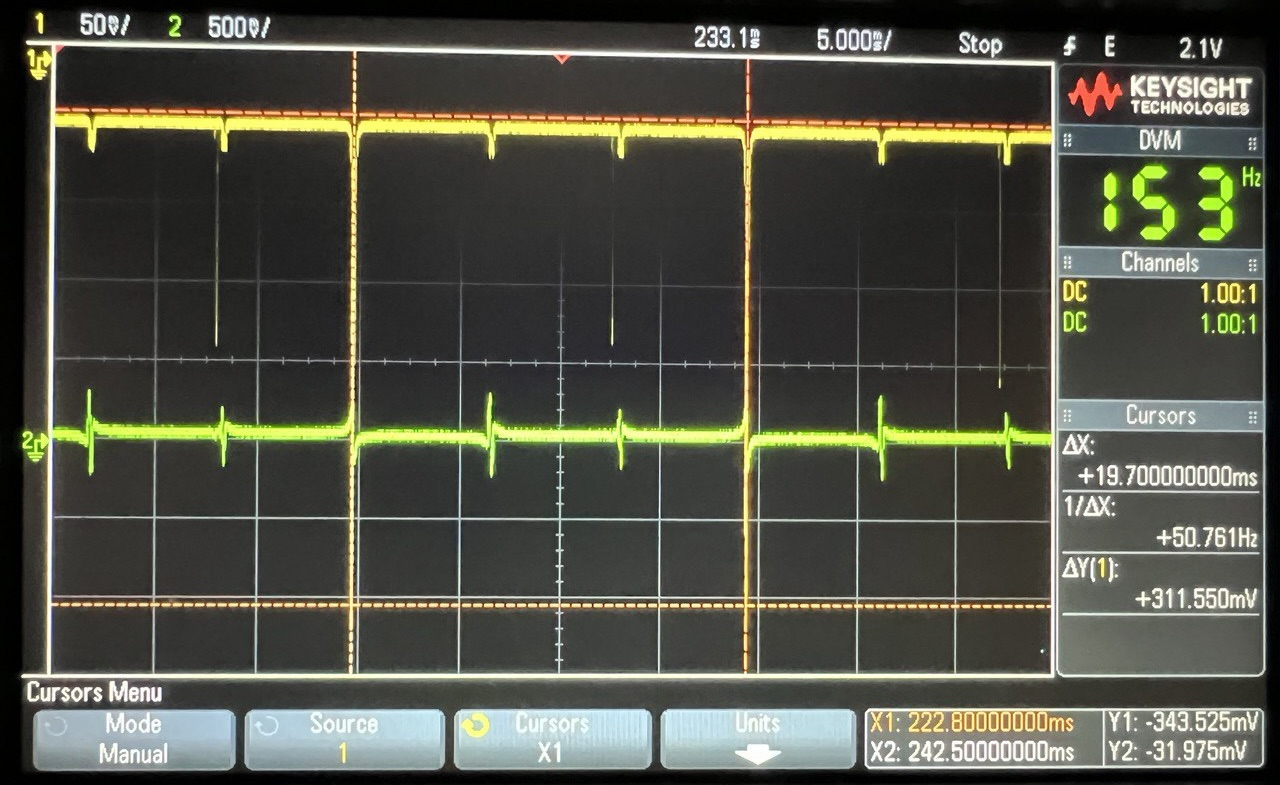
\includegraphics[width=0.45\textwidth]{Bilder/FSR/fsr_oszi.jpg} & 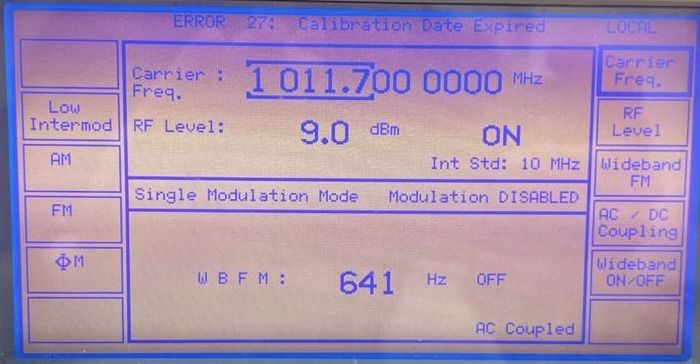
\includegraphics[width=0.45\textwidth]{Bilder/FSR/fsr_hf-generator.jpg}
    \end{tabular}
    \caption{Messung freier Spektralbereich FSR: links Oszilloskop rechts eingestellte Frequenz  $\omega_\mathrm{m}$}
    \label{fig:specBereich}
\end{center}

\newpage
\section{Finesse}
\label{sec:finess}

Als nächster Schritt wird die Finesse $F$ bestimmt mit Hilfe von Kapitel \ref{sec:specBereich}. Dafür die Modulationsfrequenz $\omega_\mathrm{m} = 50\,\mathrm{MHz} \cdot 2\pi = 314.2\,\mathrm{MHz}$ eingestellt und von da aus die Halbwertsbreite $\delta \lambda$ und die freie Spektralbereich FSR mit dem Oszilloskop bestimmt. Daraus ergeben sich folgende Werte, wobei der Fehler der Finesse $F$ mit Fehlerfortpflanzungsgesetz berechnet wurde:
\begin{gather}
    \delta \lambda = ( 44 \pm 3)\,\mu\mathrm{s}~~~~~~\mathrm{FSR}_\mathrm{OS} = (7,9 \pm 0.5)\,\mathrm{ms}\\[0,5cm]
    \Rightarrow \boxed{F = \frac{\mathrm{FSR}_\mathrm{OS}}{\delta \lambda} = (180 \pm 17)}
\end{gather}
\vspace{2cm}
\begin{center}
    \captionsetup{type=figure}
    \begin{tabular}{c c}
        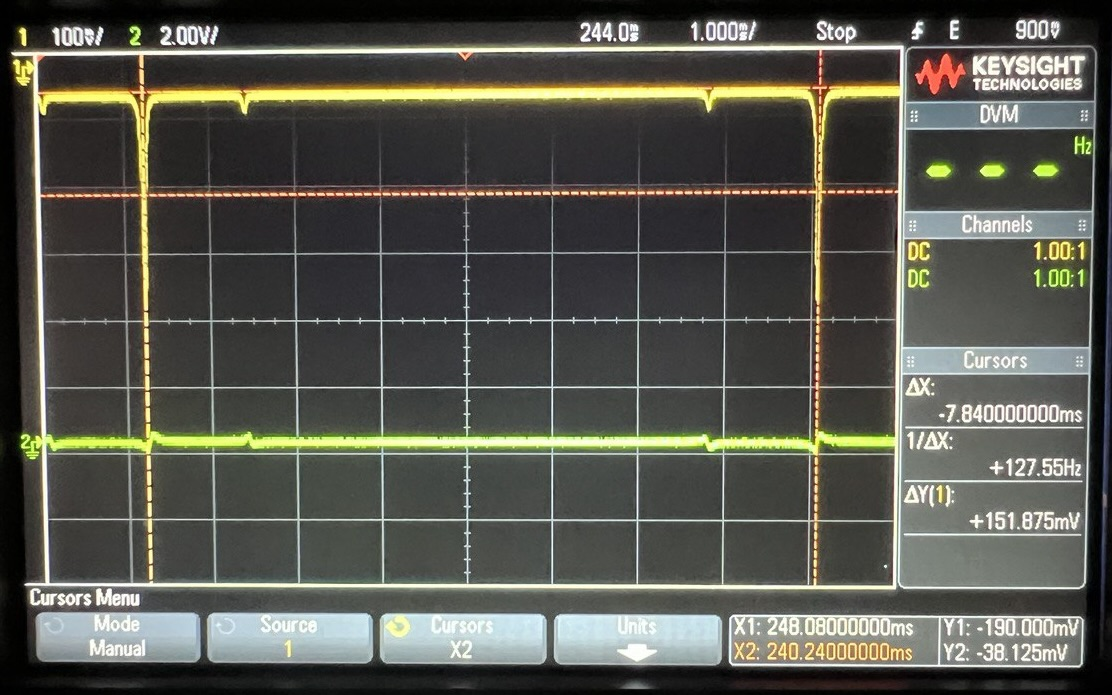
\includegraphics[width=0.45\textwidth]{Bilder/Finess/finess_fsr_oszi.jpg} & 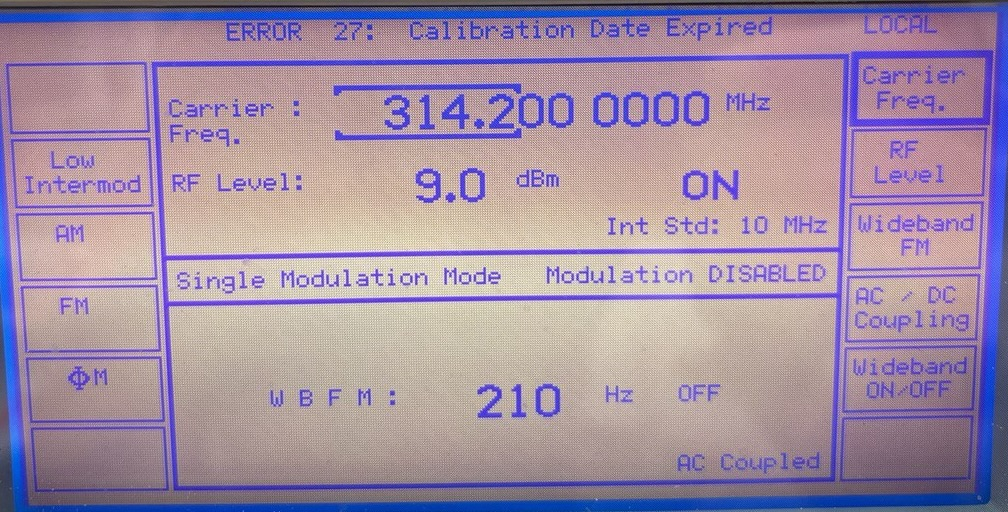
\includegraphics[width=0.45\textwidth]{Bilder/Finess/finess_hf-generator.jpg}\\
        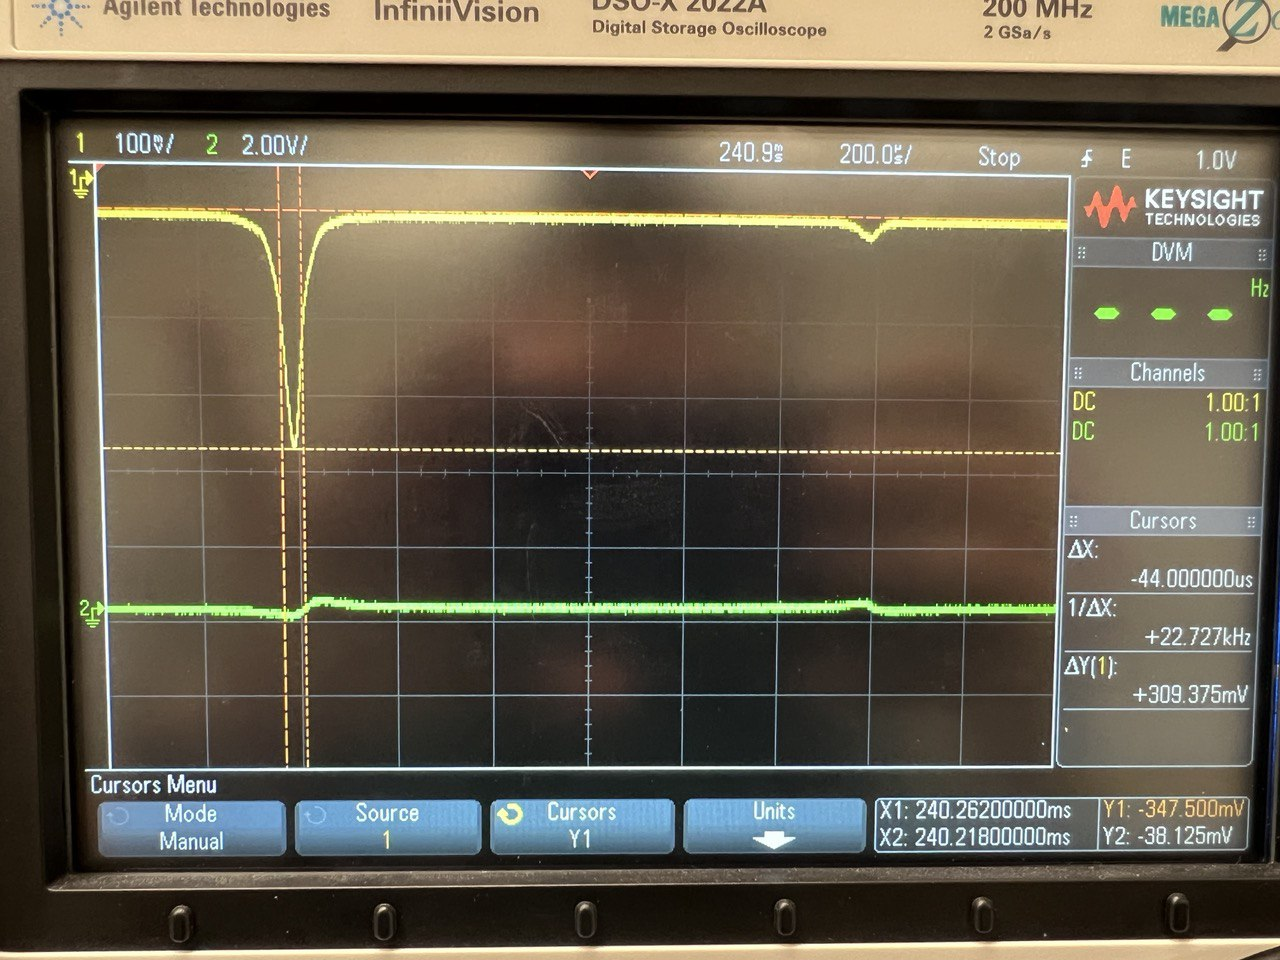
\includegraphics[width=0.45\textwidth]{Bilder/Finess/finess_max_oszi.jpg} & 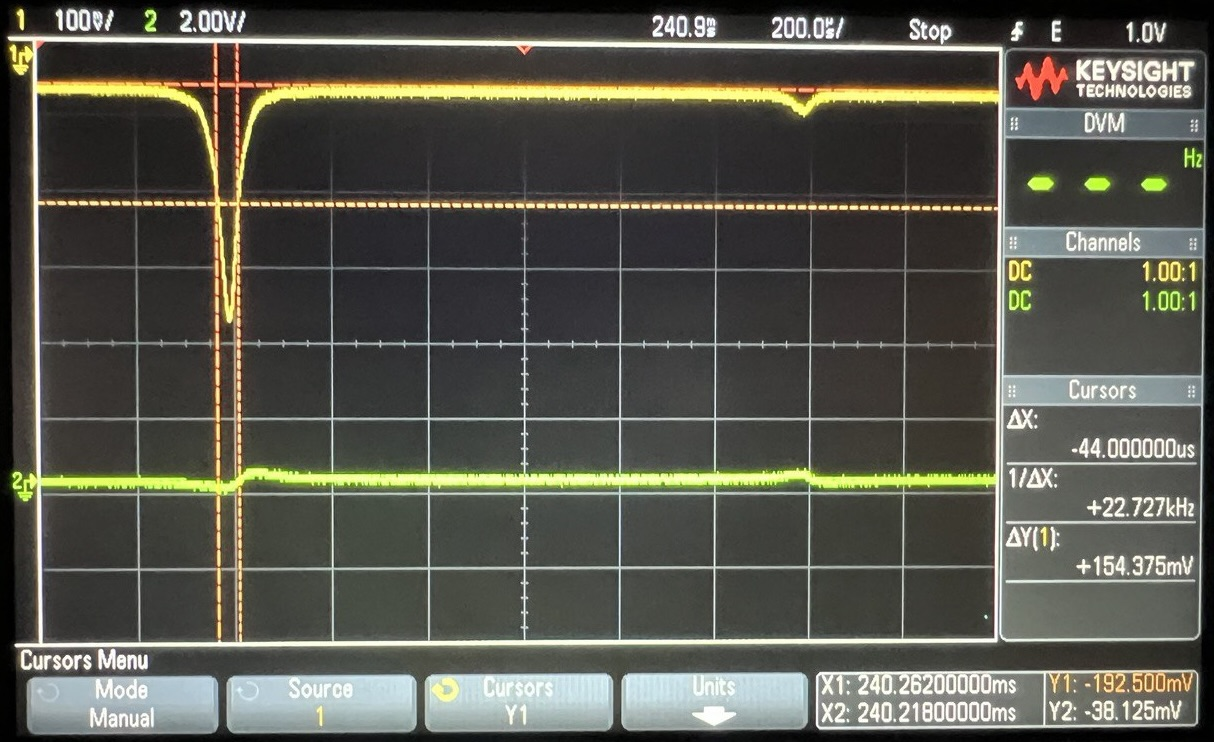
\includegraphics[width=0.45\textwidth]{Bilder/Finess/finess_hb_oszi.jpg}\\
    \end{tabular}
    \caption{Messung Finesse $F$:\\
    oben rechts: Messung des freien Spektralbereichs FSR\\
    oben links: Eingestellte Frequenz  $\omega_\mathrm{m}$\\
    unten rechts: Messung des Peaksmaximum\\
    unten links: Messung der Halbwertsbreite $\delta \lambda$}
    \label{fig:finess}
\end{center}

\newpage
\section{Modulationsindex}
\label{sec:mindex}

Als nächstes wird der Modulationsindex $M$ bei unterschiedlichen Modulationsfrequenz $\omega_\mathrm{m}$ Dabei werden folgende Werte in Tab. \ref{tab:mindex} eingestellt und daraus die Höhe aus dem Spektrum mit dem Oszilloskop abgelesen. Beachte, dass $\omega_\mathrm{m} = 0$\,MHz den ausgeschalteten HF-Generator darstellt. Der Modulationsindex wird gemäß der folgenden Formel berechnet:
\begin{gather}
    M = \frac{U(\omega_\mathrm{m})}{U(\omega_\mathrm{m} = 0)}
\end{gather}
\begin{center}
    \captionsetup{type=table}
    \begin{tabular}{r | c c}
        $\omega_\mathrm{m}$/MHz & $U$/mV & $M$ \\ \hline
        0    & 346 $\pm$ 5 & --- \\
        50   & 303 $\pm$ 5 & 0,88 $\pm$ 0,02 \\
        200  & 294 $\pm$ 5 & 0,86 $\pm$ 0,02 \\
        400  & 299 $\pm$ 5 & 0,87 $\pm$ 0,02 \\
        600  & 293 $\pm$ 5 & 0,85 $\pm$ 0,02 \\
        800  & 309 $\pm$ 5 & 0,90 $\pm$ 0,02 \\
        1000 & 313 $\pm$ 5 & 0,91 $\pm$ 0,02 \\
        1200 & 309 $\pm$ 5 & 0,90 $\pm$ 0,02 \\
        1350 & 314 $\pm$ 5 & 0,91 $\pm$ 0,02 \\
    \end{tabular}
    \captionof{table}{Werte für Modulationsindex $M$}
    \label{tab:mindex}
\end{center}

\begin{center}
    \captionsetup{type=figure}
    \begin{tabular}{c c}
        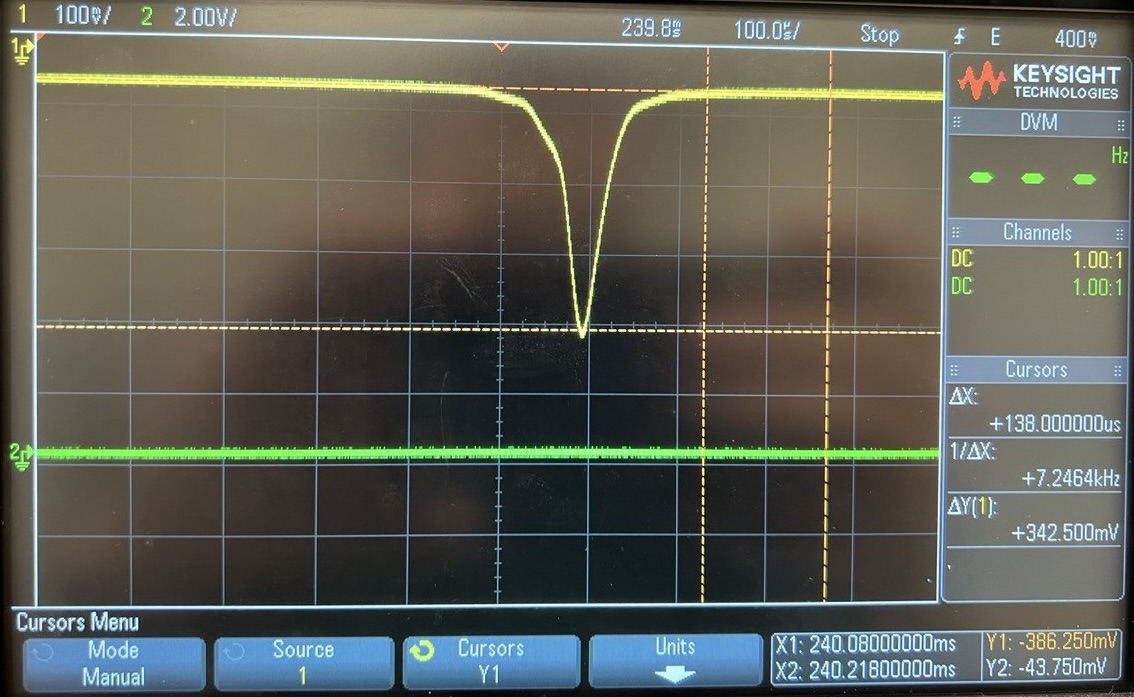
\includegraphics[width=0.45\textwidth]{Bilder/Modulationsindex/mindex_0.jpg} 
        & 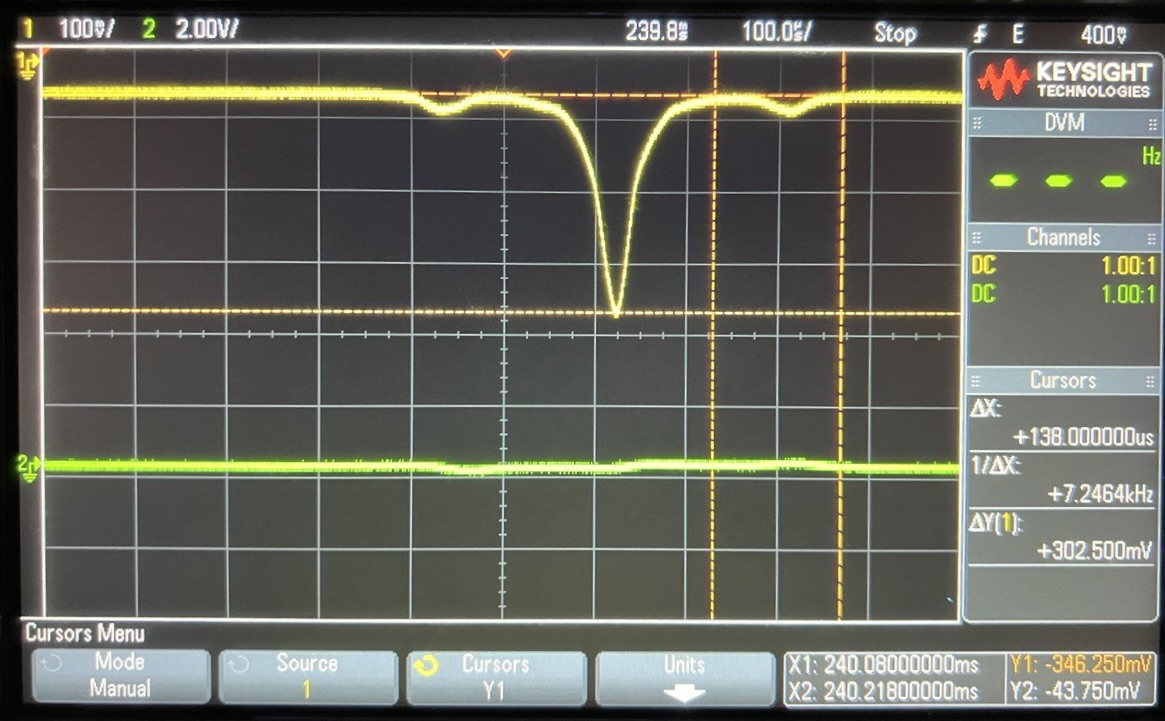
\includegraphics[width=0.45\textwidth]{Bilder/Modulationsindex/mindex_50.jpg}   \\
        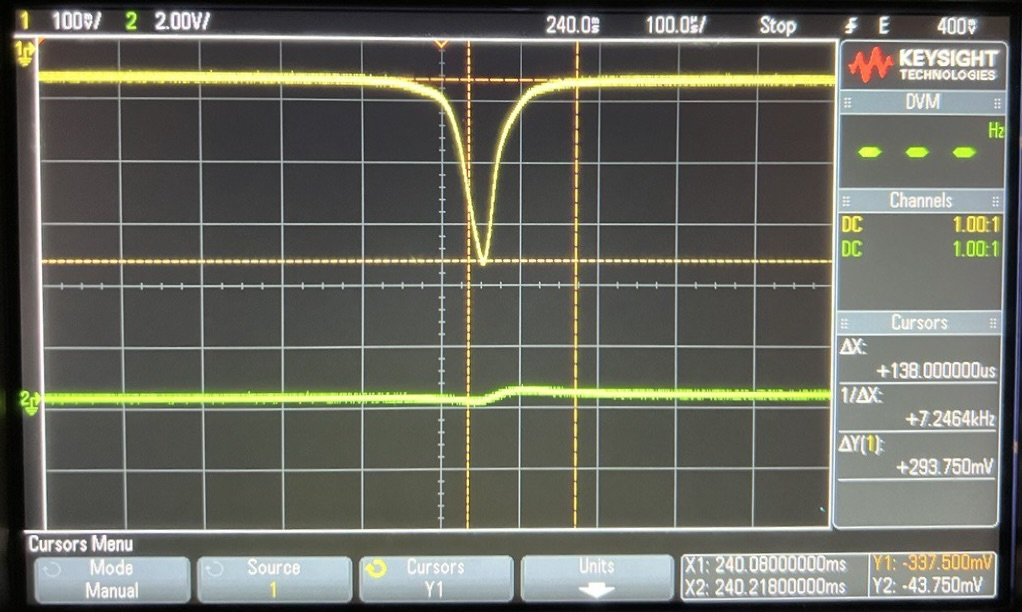
\includegraphics[width=0.45\textwidth]{Bilder/Modulationsindex/mindex_200.jpg} 
        & 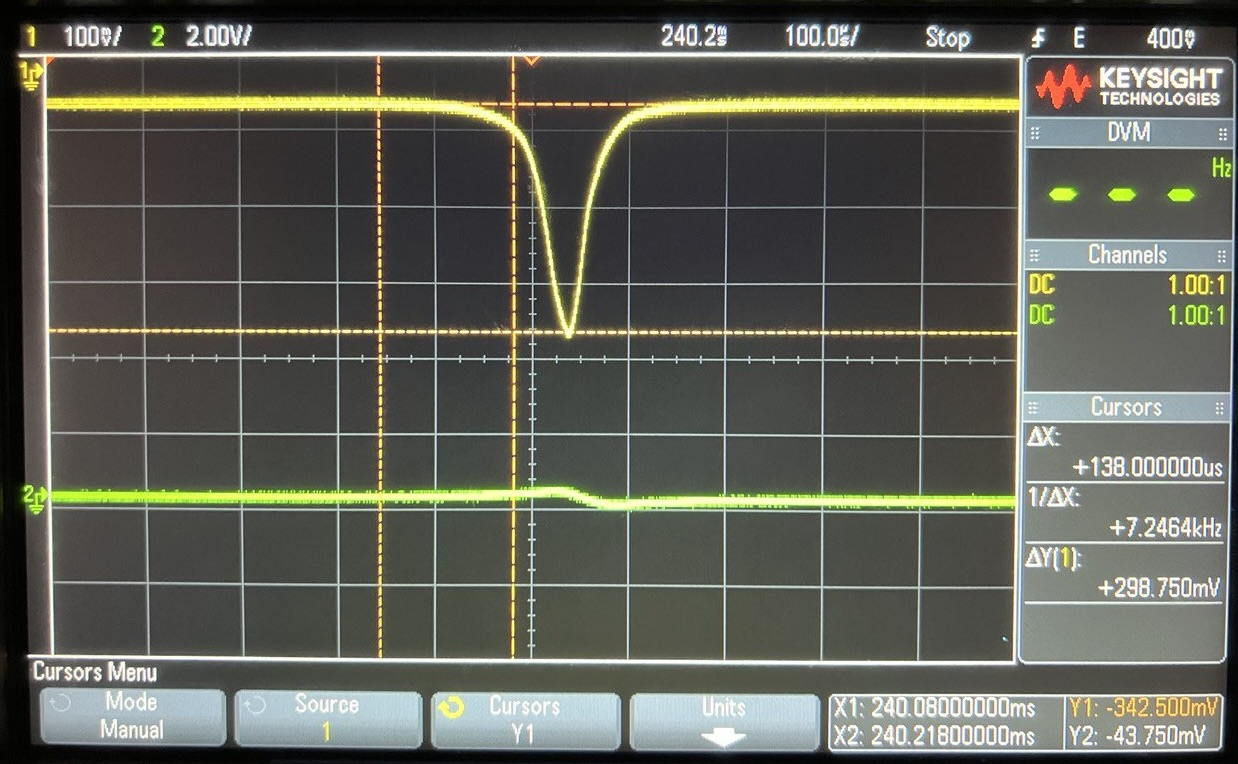
\includegraphics[width=0.45\textwidth]{Bilder/Modulationsindex/mindex_400.jpg}  \\
    \end{tabular}
    \captionof{figure}{Messung Modulationsindex $M$ für $\omega_\mathrm{m} = 0, 50, 200, 400$\,Mhz (von oben nach unten)}
    \label{fig:mindex1}
\end{center}

\begin{center}
    \captionsetup{type=figure}
    \begin{tabular}{c c}
        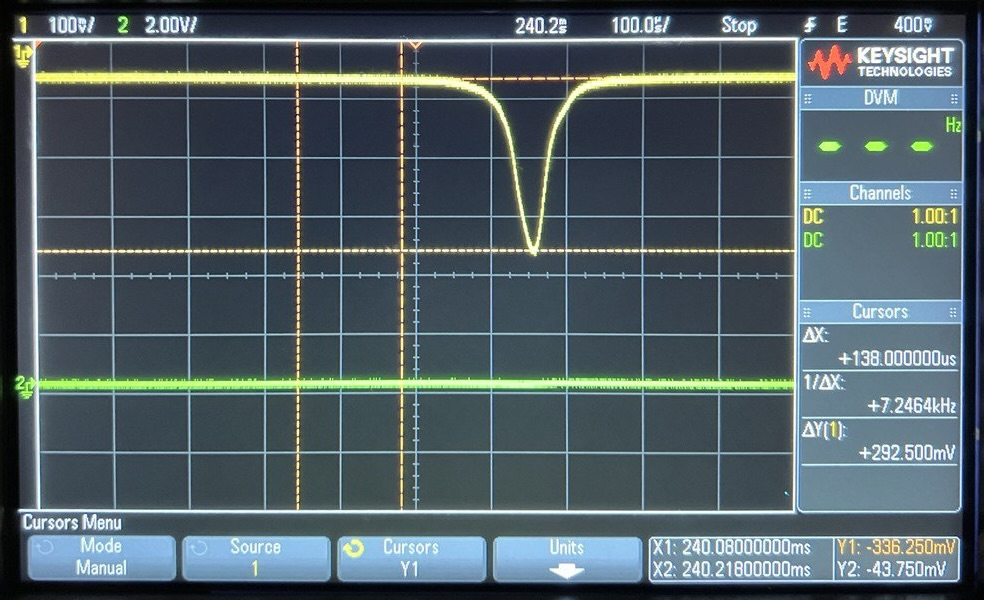
\includegraphics[width=0.45\textwidth]{Bilder/Modulationsindex/mindex_600.jpg} 
        & 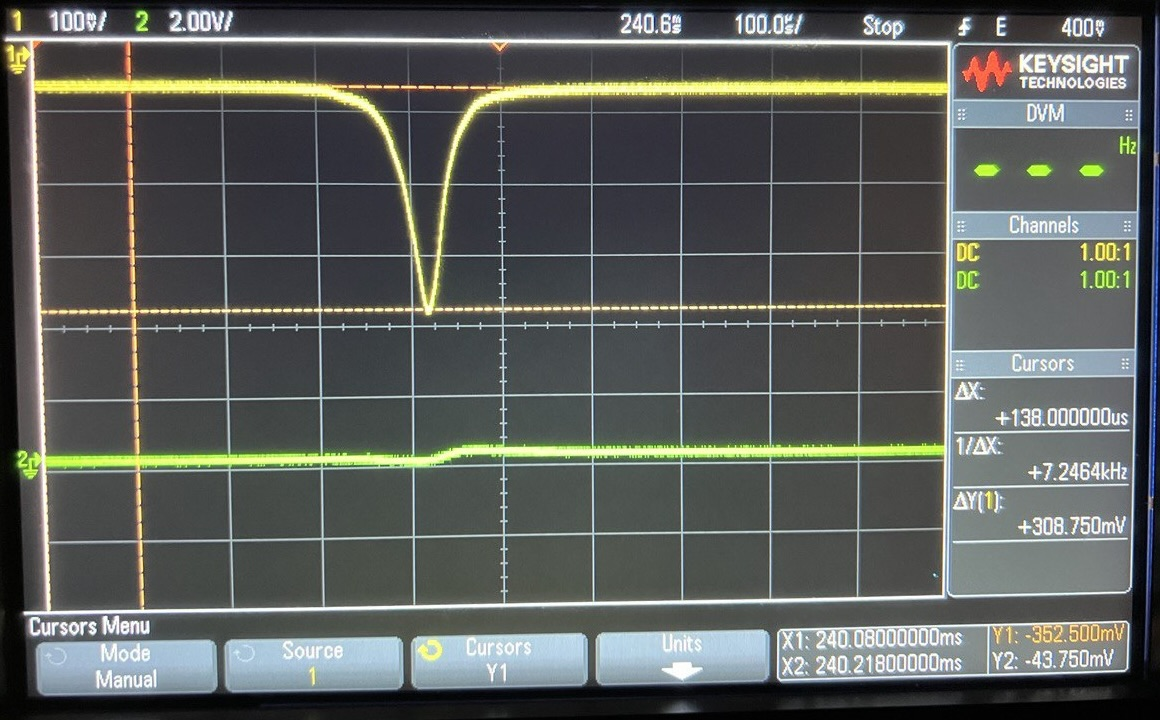
\includegraphics[width=0.45\textwidth]{Bilder/Modulationsindex/mindex_800.jpg} \\
        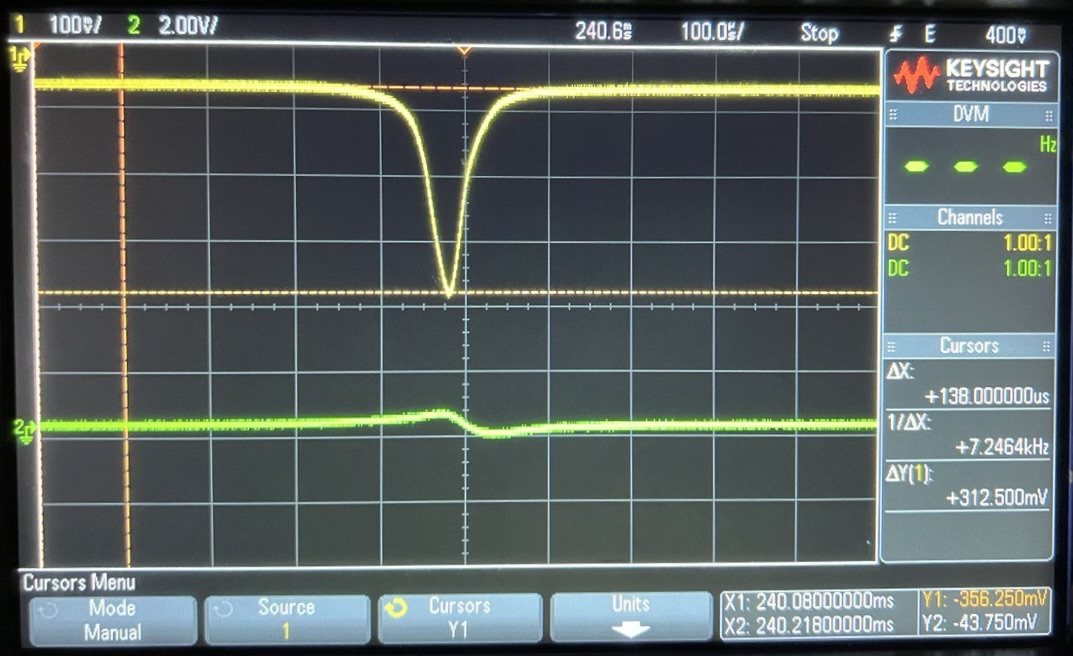
\includegraphics[width=0.45\textwidth]{Bilder/Modulationsindex/mindex_1000.jpg}
        & 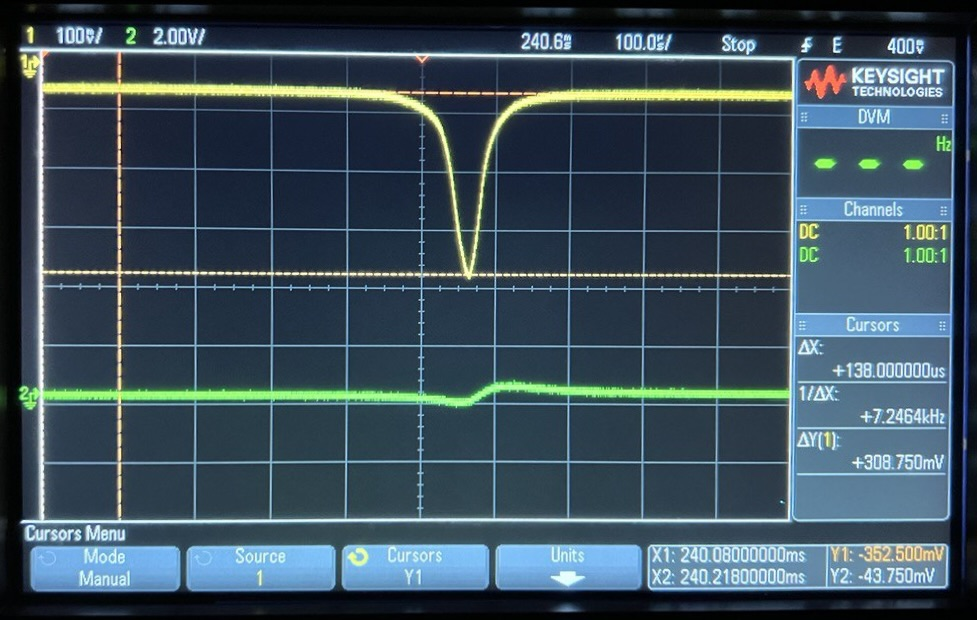
\includegraphics[width=0.45\textwidth]{Bilder/Modulationsindex/mindex_1200.jpg} \\
        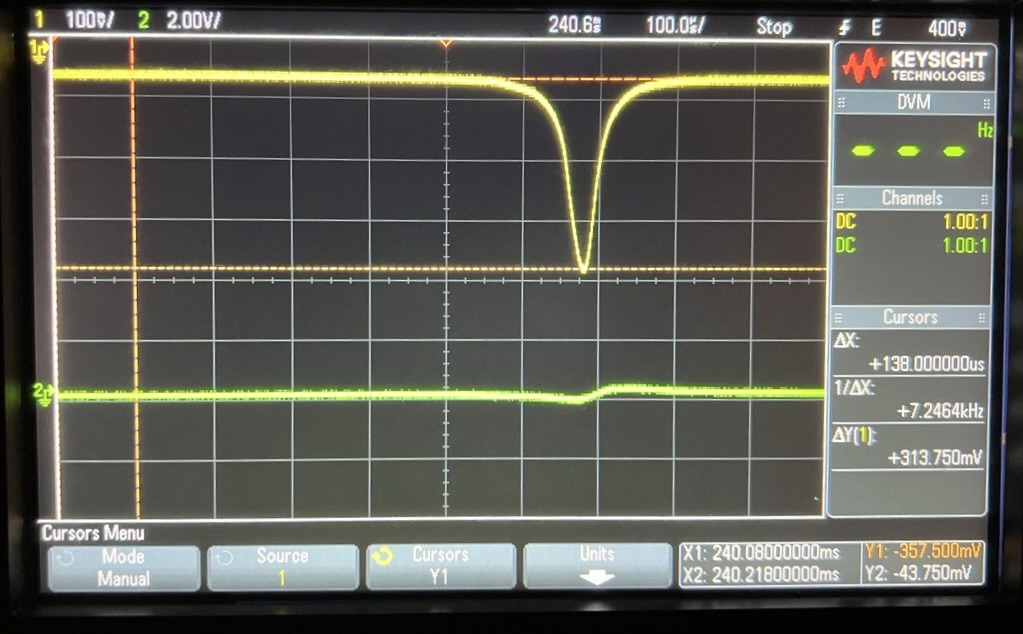
\includegraphics[width=0.45\textwidth]{Bilder/Modulationsindex/mindex_1350.jpg}
    \end{tabular}
    \captionof{figure}{Messung Modulationsindex $M$ für $\omega_\mathrm{m} = 600, 800, 1000, 1200, 1350$\,Mhz (von oben nach unten)} 
    \label{fig:mindex2}
\end{center}

\newpage

\section{Empfindlichkeit und Signal-Rausch-Verhältnis der Apparatur}
\label{sec:signalRausch}

\subsection{Optische Dichte OD}
\label{sub:opDichte}

In diesem Abschnitt berechnen wir die optische Dichte OD des Etalons. Hierfür wurden die Photodiode 3 angeschlossen, welche das Reflexionssignal des Etalons misst. Dabei ergeben sich folgende Werte mit Fehler aus Fehlerfortpflanzungsgesetz:
\begin{gather}
    U_0 = (110 \pm 5)\,\mathrm{mV}, ~~~U = (89 \pm 5)\,\mathrm{mV}\\[0,5cm]
    \Rightarrow \boxed{\mathrm{OD} = \log_{10}\left(\frac{U_0}{U}\right) = 0,09 \pm 0,07}
\end{gather} 

\begin{center}
    \captionsetup{type=figure}
    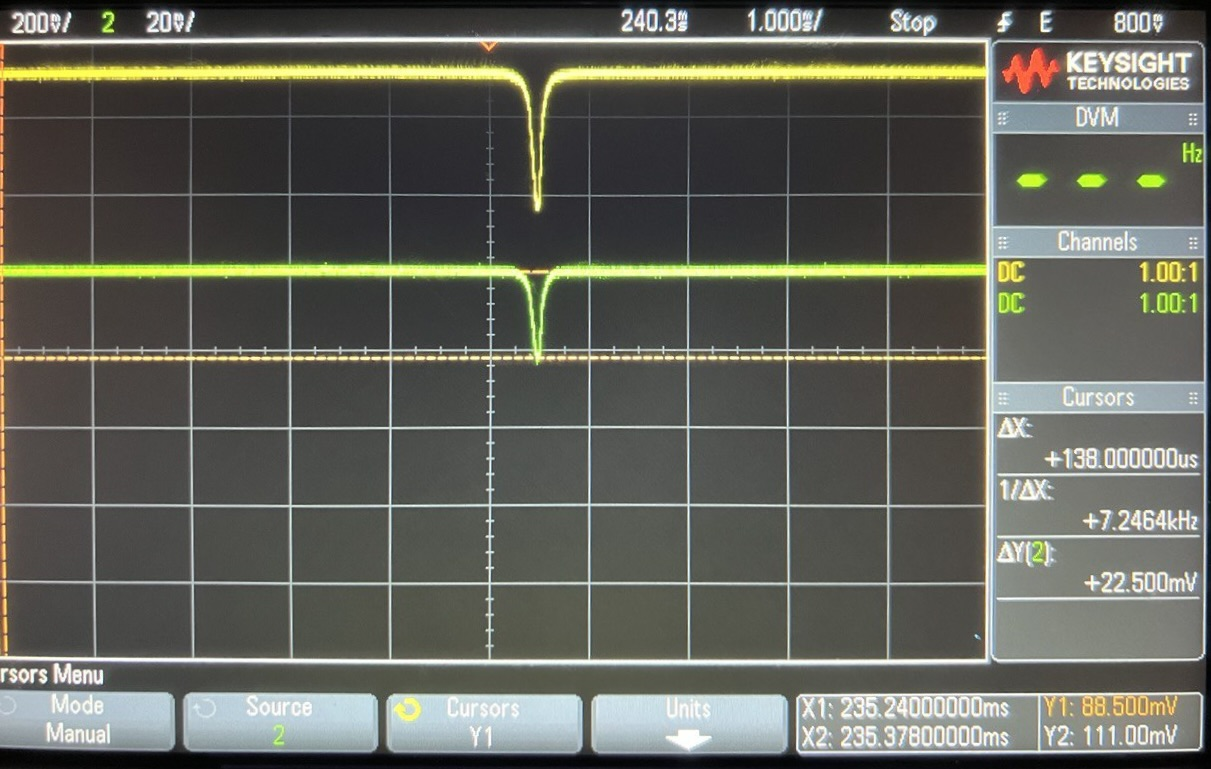
\includegraphics[scale=0.2]{Bilder/Signal-Rausch/signal-rausch_od.jpg}
    \captionof{figure}{Messung optische Dichte OD}
    \label{fig:opDichte}
\end{center}

\subsection{Bestimmung der spektrale Breite}
\label{sub:specBreite}

Das Signal wird verrauscht aufgrund der fehlenden phasensentiven Detektion des Lock-In Verstärkers. Um die spektrale Breite $\Delta \Omega$ zu bestimmen wird ein Signal aus Ref Paper (S3 Tabelle) mit den Wert $\Delta R = 5,0$ reproduziert, dazu wird erst ein Signal für $\Delta R > 5,0$ und dann das Signal ungefähr bis zum Signal  $\Delta R = 5,0$ verstellt. Aus Ref (Paper) ist bekannt:
\begin{gather}
    \Delta R = \frac{2 \omega_\mathrm{m}}{\Delta \Omega} \Leftrightarrow \Delta \Omega = \frac{2 \omega_\mathrm{m}}{\Delta R}~.
\end{gather}
Gemessen wurde die Modulationsfrequenz $\omega_\mathrm{m} = 27,3$\,MHz was dann folgende spektrale Breite ergibt: 
\begin{gather}    
    \Rightarrow \boxed{\Delta \Omega = 10,9\,\mathrm{MHz}}~.
\end{gather}
Bilder gespeichert in Datei: \textit{scope\_1}, \textit{scope\_2}

\begin{center}
    \captionsetup{type=figure}
    \begin{tabular}{c c}
        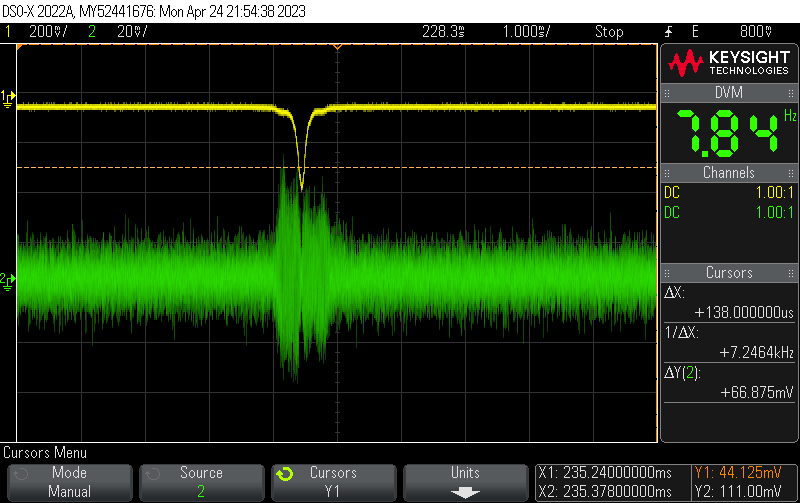
\includegraphics[scale=0.25]{Bilder/Signal-Rausch/scope_2.png} & 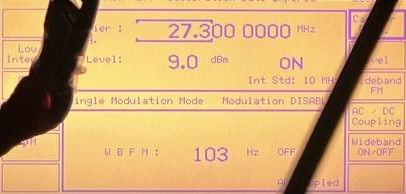
\includegraphics[width=0.45\textwidth]{Bilder/Signal-Rausch/signal-rausch_paper_hf-generator.jpg}
    \end{tabular}
    \captionof{figure}{Messung spektrale Breite $\Delta \Omega$: links Oszilloskop rechts eingestellte Frequenz  $\omega_\mathrm{m}$}
    \label{fig:specBreite}
\end{center}

\subsection{Schwebung}
\label{sub:schewbung}

Die angesprochene Schwebung konnte von den Versuchsteilnehmer nicht beobachtet werden.

\subsection{Spekturmanalysator}
\label{sub:specAnal}

Als nächstes wird das Ausgangssignal mit dem Spekturmanalysator dafür wählen wir eine Bandbreite von 10\,kHz und einen Videofilter von 100\,Hz untersucht. Dabei lesen wir die Werte der Signalhöhe $P_\mathrm{S}$ und die Höhe des Rauschpegels $P_\mathrm{R}$ von Spekturmanalysator mit dem Cursor ab, was in Tab. \ref{tab:specAnal} dokumentiert wurde.
\begin{center}
    \captionsetup{type=table}
    \begin{tabular}{r | c c}
        $\omega_\mathrm{m}$/MHz & $P^*_\mathrm{S}$/dBm & $P^*_\mathrm{R}$/dBm \\ \hline
        50   & -30 $\pm$ 3 & -80 $\pm$ 3 \\
        200  & -30 $\pm$ 3 & -80 $\pm$ 3 \\
        400  & -23 $\pm$ 3 & -80 $\pm$ 3 \\
        600  & -20 $\pm$ 3 & -77 $\pm$ 3 \\
        800  & -21 $\pm$ 3 & -77 $\pm$ 3 \\
        1000 & -20 $\pm$ 3 & -77 $\pm$ 3 \\
        1200 & -19 $\pm$ 3 & -77 $\pm$ 3 \\
        1350 & -18 $\pm$ 3 & -77 $\pm$ 3 \\
    \end{tabular}
    \captionof{table}{Werte von der Messung am Spekturmanalysator}
    \label{tab:specAnal}
\end{center}
Wenn man das Signal des Lasers abblockt verändert sich hierbei der Rauschpegel \textbf{nicht}.

\newpage

\subsection{Konversionsverluste des Mischers}
\label{sub:verluste}

In diesem Abschnitt messen wir die Konversionsverluste des Mischers. Hierfür stellen wir eine Modulationsfrequenz $\omega_\mathrm{m}$ nahe der Werte aus Kapitel \ref{sub:specAnal} liegen und lesen den Wert der Basislinie zu Spitze $U$ vom Oszilloskop ab. Dabei wird der \textbf{SWEEP} und der \textbf{OFFSET} so variiert, dass nur noch ein vollständiger Peak zu sehen ist [Abb. \ref{fig:verluste}].

\begin{center}
    \captionsetup{type=table}
    \begin{tabular}{r | c }
        $\omega_\mathrm{m}$/MHz & $U$/mV \\ \hline
        54,5   & 208 $\pm$ 5 \\
        188,5  & 293 $\pm$ 5 \\
        409,2  & 421 $\pm$ 5 \\
        629,1  & 511 $\pm$ 5 \\
        824,1  & 452 $\pm$ 5 \\
        989,0  & 533 $\pm$ 5 \\
        1235,1 & 635 $\pm$ 5 \\
        1344,5 & 572 $\pm$ 5 \\
    \end{tabular}
    \captionof{table}{Werte von der Messung der Konversionsverluste}
    \label{tab:verluste}
\end{center}

Bild gespeichert in Datei: \textit{scope\_3}

\begin{center}
    \captionsetup{type=figure}
    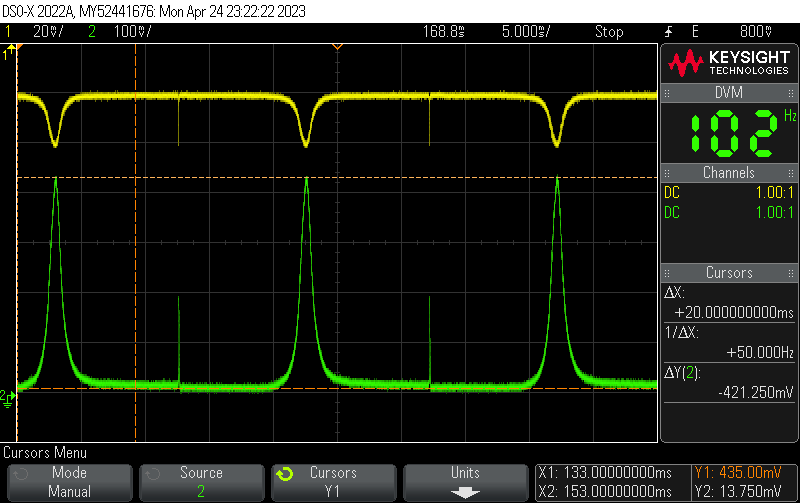
\includegraphics[scale=0.3]{Bilder/Signal-Rausch/scope_3.png}
    \captionof{figure}{Beispielmessung für die optische Dichte OD}
    \label{fig:verluste}
\end{center}

\newpage

\section{Absorptions- und Dispersionssignal einer Jodlinie}
\label{sub:jodline}

Für die Absorptions- und Dispersionssignal einer Jodlinie wird zuerst das Signal desEtalons von Spitze zu Spitze am Oszilloskop gemessen. Die Modulationsfrequenz $\omega_\mathrm{m}$ wird wie in Kapitel \ref{sub:verluste} gewählt. Die aufgenommenen Werte sind in Tab. \ref{tab:jodline} gegeben.
\begin{center}
    \captionsetup{type=table}
    \begin{tabular}{c c c}
    \begin{tabular}{r | r }
        $\omega_\mathrm{m}$/MHz & $U$/mV \\ \hline
        32,3   & 357,50 $\pm$ 5 \\
        54,5   & 425,00 $\pm$ 5 \\
        81,1   & 480,00 $\pm$ 5 \\
        106,3  & 495,00 $\pm$ 5 \\
        132,6  & 501,25 $\pm$ 5 \\
        161,4  & 540,00 $\pm$ 5 \\
        188,5  & 598,75 $\pm$ 5 \\
        215,4  & 655,00 $\pm$ 5 \\
        242,2  & 678,75 $\pm$ 5 \\
        270,1  & 725,00 $\pm$ 5 \\
        297,7  & 760,00 $\pm$ 5 \\
        326,0  & 795,00 $\pm$ 5 \\
        352,6  & 817,50 $\pm$ 5 \\
        380,3  & 772,50 $\pm$ 5 \\
        409,2  & 805,00 $\pm$ 5 \\
        436,5  & 892,50 $\pm$ 5 \\
    \end{tabular} &
    \begin{tabular}{r | r }
        $\omega_\mathrm{m}$/MHz & $U$/mV \\ \hline
        463,1  & 927,50  $\pm$ 5 \\
        491,7  & 980,00  $\pm$ 5 \\
        519,4  & 955,00  $\pm$ 5 \\
        546,0  & 1020,00 $\pm$ 5 \\
        573,6  & 905,00  $\pm$ 5 \\
        600,9  & 917,50  $\pm$ 5 \\
        629,4  & 955,00  $\pm$ 5 \\
        656,0  & 1087,50 $\pm$ 5 \\
        683,1  & 867,50  $\pm$ 5 \\
        711,6  & 837,50  $\pm$ 5 \\
        740,7  & 842,50  $\pm$ 5 \\
        768,6  & 1010,00 $\pm$ 5 \\
        794,6  & 985,00  $\pm$ 5 \\
        824,1  & 872,50  $\pm$ 5 \\
        851,8  & 1010,00 $\pm$ 5 \\
        879,0  & 1170,00 $\pm$ 5 \\
    \end{tabular} &
    \begin{tabular}{r | r }
        $\omega_\mathrm{m}$/MHz & $U$/mV \\ \hline
        905,6  & 1345,00 $\pm$ 5 \\
        931,5  & 1200,00 $\pm$ 5 \\
        960,3  & 1004,00 $\pm$ 5 \\
        989,0  & 1130,00 $\pm$ 5 \\
        1015,7 & 1067,50 $\pm$ 5 \\
        1044,4 & 1052,50 $\pm$ 5 \\
        1071,4 & 1145,00 $\pm$ 5 \\
        1098,8 & 1140,00 $\pm$ 5 \\
        1125,4 & 1110,00 $\pm$ 5 \\
        1153,6 & 955,00  $\pm$ 5 \\
        1182,4 & 1090,00 $\pm$ 5 \\
        1209,0 & 1170,00 $\pm$ 5 \\
        1235,0 & 1242,50 $\pm$ 5 \\
        1261,3 & 1002,50 $\pm$ 5 \\
        1289,8 & 785,00  $\pm$ 5 \\
        1319,5 & 967,50  $\pm$ 5 \\
        1344,4 & 1092,50 $\pm$ 5 \\
    \end{tabular}
    \end{tabular}
    \captionof{table}{Werte von der Messung am Spekturmanalysator}
    \label{tab:jodline}
\end{center}

Da weiter Messung nicht eingestellt werden konnte, wurden den Versuchsteilnehmer die Messdaten der Gruppe 3 aus dem Jahr 2020 übergeben, um die Auswertung zu bewerkstelligen. Dennoch werden drei Werte per Hand gemessen, was in Tab. \ref{tab:absorp} dargestellt wurde. Dafür wird von Basis(Index B) zu Spitze (Index P) für die Referenz (Potenz Ref) und die Probe (Potenz Probe) gemessen.

\begin{center}
    \captionsetup{type=table}
    \begin{tabular}{r | r r r r | c }
        $\omega_\mathrm{m}$/MHz & $U^{\mathrm{Ref}}_B$/mV & $U^{\mathrm{Ref}}_P$/mV & $U^{\mathrm{Probe}}_B$/mV & $U^{\mathrm{Probe}}_P$/mV & Datei \\ \hline
        79,7   & 3 $\pm$ 3 & 131 $\pm$ 3 & 3 $\pm$ 3 & 133 $\pm$ 3  & scope\_6, scope\_7 \\
        491,9  & 1 $\pm$ 3 & 269 $\pm$ 3 & -149 $\pm$ 3 & 121 $\pm$ 3 & scope\_4, scope\_5 \\
        989,1  & -18 $\pm$ 3 & 265 $\pm$ 3 & -338 $\pm$ 3 & -18 $\pm$ 3 & scope\_8, scope\_9 \\
    \end{tabular}
    \captionof{table}{Werte von der Messung Absorption}
    \label{tab:absorp}
\end{center}

\begin{center}
    \captionsetup{type=figure}
    \begin{tabular}{c c}
        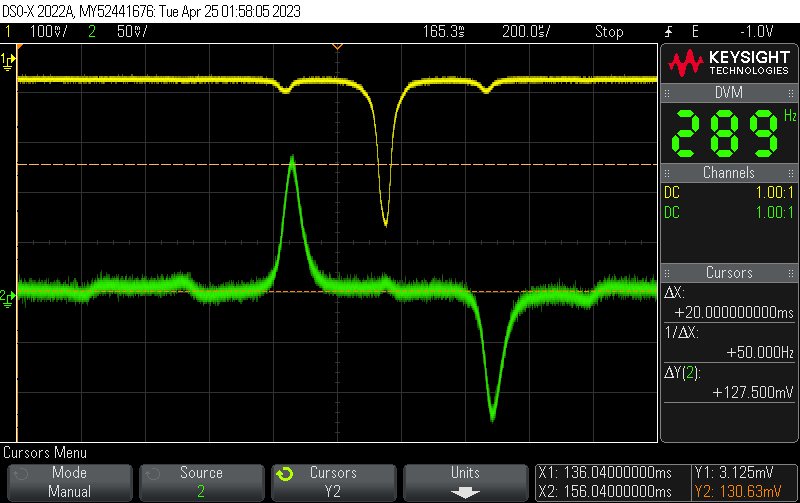
\includegraphics[width=0.45\textwidth]{Bilder/Jodlinie/scope_6.png} 
        & 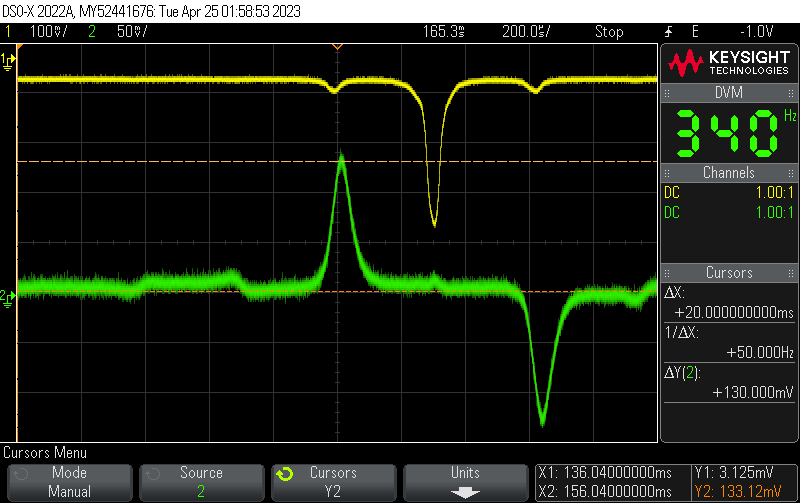
\includegraphics[width=0.45\textwidth]{Bilder/Jodlinie/scope_7.png} \\
        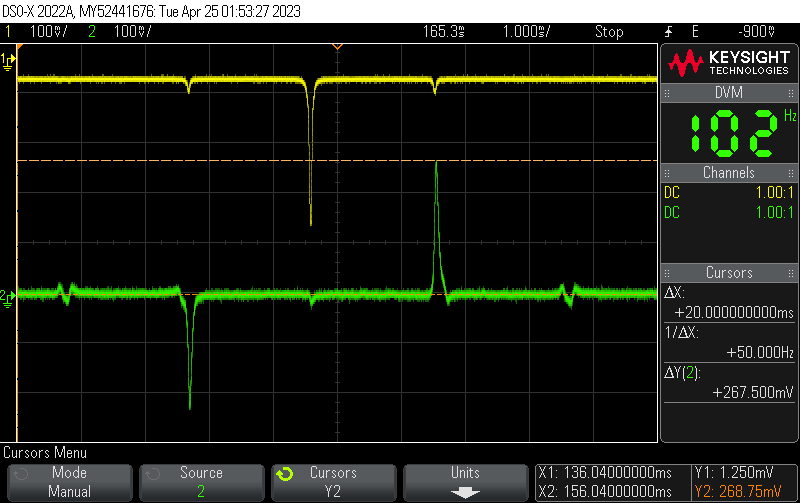
\includegraphics[width=0.45\textwidth]{Bilder/Jodlinie/scope_4.png}
        & 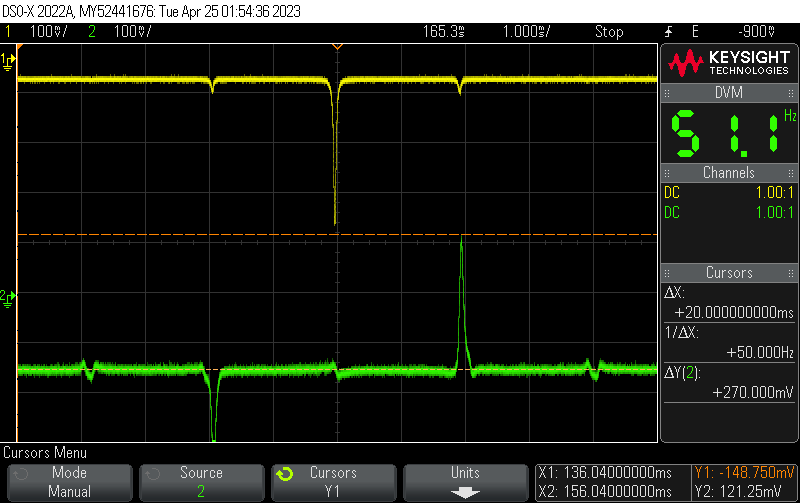
\includegraphics[width=0.45\textwidth]{Bilder/Jodlinie/scope_5.png} \\
        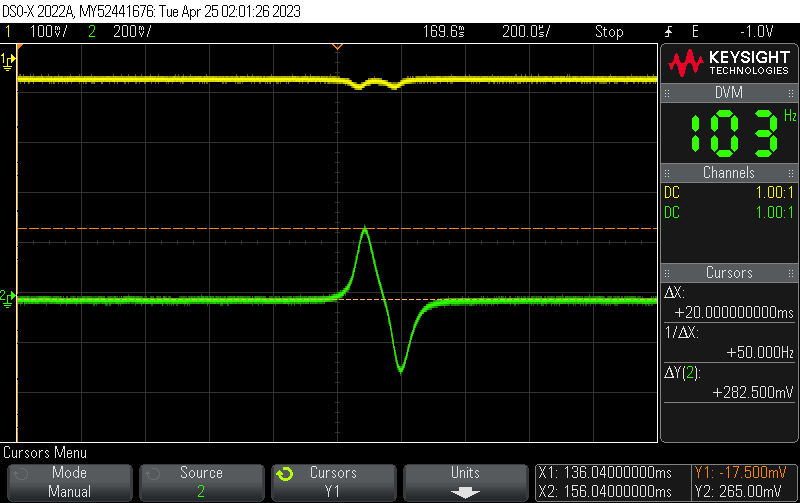
\includegraphics[width=0.45\textwidth]{Bilder/Jodlinie/scope_8.png}
        & 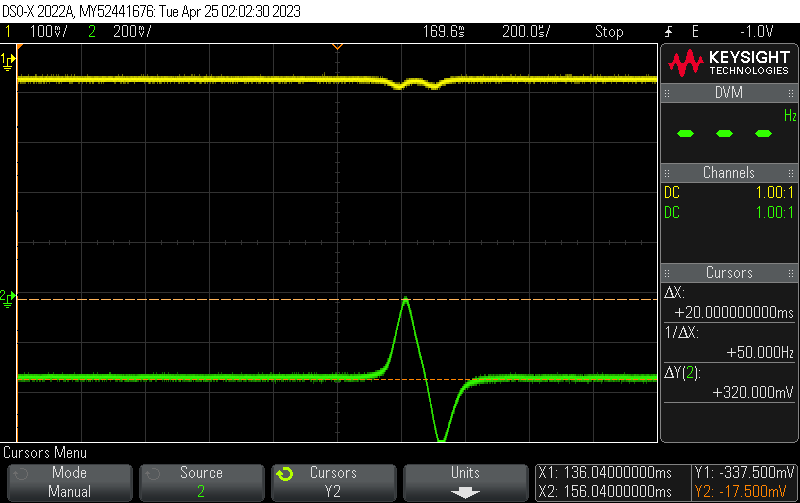
\includegraphics[width=0.45\textwidth]{Bilder/Jodlinie/scope_9.png}
    \end{tabular}
    \captionof{figure}{Messung der Absorption rechts Referenz links Probe für $\omega_\mathrm{m} $ = 79,7; 491,9; 989,1\,Mhz (von oben nach unten)}
    \label{fig:absorp}
\end{center}

%Das Messprotokoll wurde am Versuchstag handschriftlich erstellt und hier als
%PDF-Datei eingefügt. Dabei wurden Durchführung und Aufbau schon vorher in dieses
%Dokument beschrieben, je nachdem.

% Einbindung des Protokolls als pdf (mit Seitenzahl etc.)
% Erste Seite mit Überschrift
%\includepdf[pages = 1, landscape = false, nup = 1x1, scale = \skalierung , pagecommand={\thispagestyle{empty}\chapter{Protokoll}}]
%            {03-Protokoll/Protokoll.pdf}
% Restliche Seiten richtig skaliert
%\includepdf[pages = -, landscape = false, nup = 1x1, scale = \skalierung , pagecommand={}]
%            {03-Protokoll/Protokoll.pdf}